\documentclass[11pt,letterpaper]{article}
\usepackage{times}
\usepackage[onehalfspacing]{setspace}
% bibliography
\usepackage{natbib}\bibpunct{(}{)}{,}{}{}{,}
\bibliographystyle{bib/aeaown}

\usepackage{amsmath,amsfonts,amsthm}
\usepackage{comment}
\usepackage{tabularx}
\usepackage{multirow}
\usepackage{booktabs}
\usepackage{subcaption}
\usepackage{graphicx}
\usepackage[colorlinks,linkcolor=blue,citecolor=black,urlcolor=black]{hyperref}
\usepackage[title,titletoc]{appendix}
\usepackage{enumitem}
\usepackage{subcaption}  % For subfigures
\usepackage{lscape}      % For landscape orientation if needed
\usepackage[noabbrev,capitalize]{cleveref}
\usepackage{pgfplots}
\pgfplotsset{compat=1.18}
\usepackage{amsmath}
\usepackage{tikz}
\usetikzlibrary{patterns, decorations.pathreplacing}

% commands
\newtheorem{definition}{Definition}
\newtheorem{proposition}{Proposition}
\newtheorem{lemma}{Lemma}
\newtheorem{assumption}{Assumption}
\newcommand{\figpath}{fig/}
\newcommand{\tablepath}{table/}
\newcommand{\rmdi}{\mathrm{d}}

% table and figure formatting
%\input{formats}

% page size
\setlength{\textwidth}{\paperwidth}
\addtolength{\textwidth}{-1.7in}
\setlength{\oddsidemargin}{.85in}
\addtolength{\oddsidemargin}{-.85in}
\setlength{\evensidemargin}{\oddsidemargin}
\setlength{\headheight}{0pt}
\setlength{\headsep}{0pt}
\setlength{\textheight}{\paperheight}
\addtolength{\textheight}{-\headheight}
\addtolength{\textheight}{-\headsep}
\addtolength{\textheight}{-\footskip}
\addtolength{\textheight}{-1.75in}
\setlength{\topmargin}{1in}
\addtolength{\topmargin}{-1in}

\begin{document}

\title{\textbf{A Simple Theory of Trade Rerouting}}
\author{\large%
\setcounter{footnote}{0}%
%Carlos G\'{o}es \\[-3pt] \textit{\small World Bank Group}%
}
\date{\today}
\maketitle

\vspace{-0.7cm}
\noindent\begin{abstract}\begin{singlespace}
\noindent xxxx
 
[4pt]\textbf{Keywords}: xx.
\\[4pt] \textbf{JEL Classification}: xx
\end{singlespace}
\end{abstract}

\newpage

\section{Environment}\label{sec:environment}
Consider a world consisting of three countries, a foreign source country $f$, a home country $h$, and an entrepot country $r$. At the destination country $h$, consumers have preferences over domestic and foreign goods:

\begin{equation*}
    C \equiv \left[ \alpha^{\frac{1}{\rho}} C_H^{\frac{\rho - 1}{\rho}} + (1 - \alpha)^{\frac{1}{\rho}} C_F^{\frac{\rho - 1}{\rho}} \right]^{\frac{\rho}{\rho - 1}}
\end{equation*}

By optimality, home consumers exhaust their income, such that $PC = P_H C_H + P_F C_F = wL$, where $L$ is the labor endowment and $P \equiv [\alpha P_H^{-(\rho-1)} + (1-\alpha) P_F^{-(\rho-1)}]^{-\frac{1}{\rho-1}}$ is the ideal price index. We set to the price of the home good $P_H=1$ be the num\'eraire of the home economy.

In the home sector, there is a representative firm endowed with a linear technology and productivity $A_H$. Households can only work in the home sector. Hence, optimal production choices determine the wage $w = A_H$. There is a domestic assembler who sources infinitely many varieties $\omega$ and combines them into a composite good using a constant returns to scale technology:

\begin{equation*}
    Y_F = \left[ \int_0^1 y(\omega)^{\frac{\sigma-1}{\sigma}} d\omega \right]^\frac{\sigma}{\sigma-1}
\end{equation*}

Assemblers can source an identical variety $\omega$ through one of two ways. They can buy them directly from the foreign country, paying prices $p_{fh}(\omega)$; or they can buy them from the rerouting country, paying price $p_{rh}(\omega)$. Since varieties are identical, they will source each variety from the cheapest possible alternative, such that $p(\omega) = \min \{p_{fh}(\omega),p_{rh}(\omega) \}$. By cost minimization, demand for each variety satisfies:
\begin{equation}\label{eq: optimal-demand}
    q(\omega) = \left( \frac{p(\omega)}{P_F} \right)^{-\sigma} \times P_F C_F
\end{equation}
Trade in this economy is not costless. Varieties are subject to iceberg trade costs, meaning that for one unit of good $\omega$ produced at $f$ to arrive at $r$, $\tau_{fr}(\omega) \ge 1$ need to be produced. Similarly, for a good from $r$ to arrive at $h$, $\tau_{rh}(\omega) \ge 1$ need to be shipped. We call $\tau^R_{fh}(\omega) \equiv \tau_{fr}(\omega) \tau_{rh}(\omega)$ the trade cost of rerouting good $\omega$. Note that we allow them to be good-specific rather than uniformly applied for all goods.

At the rerouting country, there are traders with exclusive rights over each variety $\omega$. Taking as a given the demand at $h$, traders source each variety paying price $p_{fr}(\omega)$ and sell it to the home country. The optimal price for traders is the standard markup over marginal cost:

\begin{equation}\label{eq: trader-price}
    p_{rh}(\omega) = \mu \times \tau_{rh}(\omega) \times p_{fr}(\omega)
\end{equation}

\noindent where $\mu \equiv \frac{\sigma}{\sigma-1}$ is the markup. Shipping from the foreign country to the home country is also subject to iceberg costs $\lambda \times \tau_{fh}(\omega)$, where $\lambda$ is some arbitrary scaling factor that rotates the trade cost schedule. To produce a single unit of variety $\omega$, producers incur a marginal cost $c_f$, taken as exogenous. 

When selling the good to $r$, producers will take optimal demand in $r$ as given, and choose prices $p_{fr}(\omega)$ to maximize profits. Traders in $r$ will buy exactly the amount goods that they will sell to $h$, net of trade costs, thereby maximizing their profits. Replacing  optimal trader prices \eqref{eq: trader-price} into demands functions \eqref{eq: optimal-demand}, demand in $r$ for variety $\omega$ will be:

\begin{equation*}
    q(\omega) = \left( \frac{\mu \times \tau_{rh}(\omega) \times p_{fr}(\omega)}{P_F} \right)^{-\sigma} \times P_F C_F
\end{equation*}

It turns out that the solution to this problem is identical to the standard monopolistic competition problem, since the additional terms within the demand function do not depend on the producers choice of prices. Hence, prices satisfy $p_{fr}(\omega) = \mu \times \tau_{fr}(\omega) \times c_f$. If the producer is shipping the good from $f$ directly to $h$, then it solves a standard monopolistic competition problem and prices will be $p_{fh}(\omega) = \mu \times \lambda \times \tau_{fh}(\omega) \times c_f$. Therefore, prices at the home country satisfy:

\begin{equation}\label{eq: home-price}
    p(\omega)  = \min \{ p_{fh}(\omega) , p_{rh}(\omega) \} = \min \{  \lambda \times \tau_{fh}(\omega),  \mu \times \tau^R_{fh}(\omega) \}  \times\mu  \times c_f
\end{equation}

For the home consumer,  there is a clear benefit of rerouting. In the absence of rerouting, prices would be weakly higher. But that benefit comes at a price. Note that whenever goods arrive through rerouting, both the producer and the trader charge their own markup $\mu$, such that the rerouted price is $p_{rh}(\omega) = \mu^2 \times \tau^R_{fh}(\omega)  \times c_f$. In the industrial organization literature, this is called ``double marginalization,'' which is an additional inefficiency relative to the standard monopolistic competition problem. In the trade literature, this feature mirrors models of trade with intermediaries, such as \citet{crozet_wholesalers_2013} and \citet{ahn_role_2011}. We will later explore how vertical integration can minimize this inefficiency and maximize the gains from rerouting. 

%This model explicitly integrates insights from the industrial organization literature on double marginalization by introducing rerouting intermediaries that impose additional monopoly markups. Specifically, when goods pass through the rerouting country, they incur markups from both the foreign producers and the rerouting traders, creating inefficiencies analogous to those first characterized by Spengler (1950). This structure resonates with canonical frameworks in industrial organization, notably the detailed treatment by Tirole (1988), which emphasizes how vertical separation and successive monopolies exacerbate welfare losses. Moreover, the analysis connects directly to the trade literature focused on intermediaries, particularly the models developed by Crozet et al. (2013) and Ahn et al. (2011), which highlight similar inefficiencies arising from sequential markups in international trade. Consequently, this framework underscores the potential welfare improvements achievable through vertical integration, aligning incentives, and reducing cumulative price distortions.

\begin{assumption}[Single Crossing] \label{ass:single-crossing}  We assume that the trade cost functions are strictly decreasing, satisfying $\tau_{fh}'(\omega) < {\tau^{R}_{fh}}'(\omega) < 0$. Furthermore, we assume that for some range of goods it is less costly to ship goods directly while for some other range it is cheaper to reroute, inclusive of trader markups. Formally, we assume that $\lambda \times \tau_{fh}(0) > \mu \times  \tau^R_{fh}(0)$ and $\lambda \times \tau_{fh}(1) < \mu \times \tau^R_{fh}(1)$.
\end{assumption}

Given Assumption 1, for some $\omega^* \in [0,1]$, $\lambda \times \tau_{fh}(\omega^*) = \mu \times \tau^R_{fh}(\omega^*)$, which implies that all goods $[0, \omega^*)$ will be exported directly from $f$ to $h$ while all goods $[\omega^*,1]$ will be rerouted. The price $p(\omega)$ will be a nonconvex decreasing function, as the lower envelope of the two possible prices. This is shown on the panel \ref{fig:panelA}. What happens if there is a change in direct shipping costs, such that scaling factor now becomes $\lambda' > \lambda$? This shifts up the whole trade cost schedule. As a result, the cut-off points moves down a new range of goods $\omega \in ({\omega^*}' , \omega^*)$ will be subject to rerouting. This is shown on the panel \ref{fig:panelB}. This translates into changes in welfare and we summarize welfare effects in Proposition \ref{prop:welfare}.

\newpage

\begin{figure}[htp]
  \centering
  \begin{subfigure}[b]{0.48\textwidth}
    \centering
    \begin{tikzpicture}
    \begin{axis}[
        domain=0.01:1,
        samples=200,
        xlabel=,
        ylabel={$p(\omega)$},
        xmin=0, xmax=1,
        ymin=0, ymax=5,
        axis lines=left,
        width=\textwidth,
        height=6cm,
        smooth,
        thick,
        grid=none,
        ytick={}, yticklabels={},
        xtick={0, \wstar, 1},
        xticklabels={\(\!0\!\), \(\omega^*\), \(\!1\!\)}
    ]
    
    % Parameters: original
    \def\taufh{1.4}
    \def\taurh{1}
    \def\elasfh{0.2}
    \def\elasrh{0.6}
    % No lambda shift here
    \def\muParam{1.1}
    % Compute cutoff
    \pgfmathsetmacro{\wstar}{(\muParam * \taurh/\taufh)^(1/(\elasrh - \elasfh))}
    
    % Cost curves
    \addplot[dotted, thick] { \taufh * x^(-\elasfh) };
    \addplot[dotted, thick] { \muParam * \taurh  * x^(-\elasrh) };
    
    % Envelope and cutoff
    \addplot[solid, very thick, red]
      { min(\taufh*x^(-\elasfh),  \muParam * \taurh*x^(-\elasrh)) };
    \addplot[red, dashed, thick]
      coordinates {(\wstar,0) (\wstar,5)};
    
    \end{axis}
    \end{tikzpicture}
    \caption{Original schedule (\(\lambda=1\))}\label{fig:panelA}
  \end{subfigure}
  \hfill
  \begin{subfigure}[b]{0.48\textwidth}
    \centering
    \begin{tikzpicture}
    \begin{axis}[
        domain=0.01:1,
        samples=200,
        xlabel=,
        ylabel={$p(\omega)$},
        xmin=0, xmax=1,
        ymin=0, ymax=5,
        axis lines=left,
        width=\textwidth,
        height=6cm,
        smooth,
        thick,
        grid=none,
        ytick={}, yticklabels={},
        xtick={0, \wstar, \wstarprime, 1},
        xticklabels={\(\!0\!\), \(\omega^*\), \({\omega^*}'\), \(\!1\!\)}
    ]
    
    % Parameters: original + shifted
    \def\taufh{1.4}
    \def\taurh{1}
    \def\elasfh{0.2}
    \def\elasrh{0.6}
    \def\lambdaParam{1.2}
    \def\muParam{1.1}
    % Compute cutoffs
    \pgfmathsetmacro{\wstar}{(\muParam * \taurh/\taufh)^(1/(\elasrh - \elasfh))}
    \pgfmathsetmacro{\wstarprime}{((\muParam * \taurh)/(\lambdaParam*\taufh))^(1/(\elasrh - \elasfh))}
    
    % Cost curves
    \addplot[dotted, thick] { \taufh * x^(-\elasfh) };
    \addplot[dotted, thick] { \muParam * \taurh  * x^(-\elasrh) };
    \addplot[dotted, thick, blue]
      { (\lambdaParam*\taufh) * x^(-\elasfh) };
    
    % Envelopes and cutoffs
    \addplot[solid, very thick, red]
      { min(\taufh*x^(-\elasfh),  \muParam*\taurh*x^(-\elasrh)) };
    \addplot[solid, very thick, blue]
      { min((\lambdaParam*\taufh)*x^(-\elasfh), \muParam*\taurh*x^(-\elasrh)) };
    \addplot[red, dashed, thick]
      coordinates {(\wstar,0) (\wstar,5)};
    \addplot[blue, dashed, thick]
      coordinates {(\wstarprime,0) (\wstarprime,5)};
    
    \end{axis}
    \end{tikzpicture}
    \caption{After discrete increase (\(\lambda>1\))}\label{fig:panelB}
  \end{subfigure}
  \caption{Comparison of price schedules before and after a discrete change in \(\lambda\).}
  \label{fig:two_panels}
\end{figure}

\begin{proposition}[Welfare effects] \label{prop:welfare} Let the environment be as above and Assumption \ref{ass:single-crossing} hold. Then:

\begin{enumerate}
    \item The elasticity of welfare with respect to a shift in the direct trade cost schedule is:

    \[ \frac{d \ln C(\lambda)}{ d \ln \lambda} = - S_F(\lambda) \times s_{fh}(\lambda) \]

    where $S_F(\lambda)$ is the share of total expenditures spent on foreign goods and $s_{fh}(\lambda)$ is the share of total expenditure on foreign goods spent on goods shipped directly from $f$ to $h$.

    \item And the total cumulative welfare change is:

    \[ \ln C(\lambda') - \ln C(\lambda) =  - \int_\lambda^{\lambda'} \frac{S_F(\tilde{\lambda}) \times s_{fh}(\tilde{\lambda})}{\tilde{\lambda}}   d \tilde{\lambda}   \]
\end{enumerate}
    
\end{proposition}

\begin{proof}
    Appendix \ref{sec:proof-1}.
\end{proof}

These results are intuitive. The instantaneous effect of increasing the direct trade cost schedule will be proportional to (i) expenditure shares in foreign goods out of total expenditure; and (ii) expenditure shares in goods shipped directly from $f$ to $h$ out of total foreign goods.

At the cutoff variety $\omega^*$ the prices at $h$ of direct shipment and rerouting exactly equate $p_{fh}(\omega^*)=p_{rh}(\omega^*)$, rendering assemblers indifferent between the two routes. Thus, a small change in the direct shipping costs schedule induce a change in the prices of all inframarginal varieties $\omega \in [0,\omega^*)$ but no discrete adjustments in the cutoff variety. Consequently, expenditure shares and welfare respond continuously, resulting in smoothly evolving trade flows and welfare outcomes. 

Cumulative changes in welfare embed two effects. The costs of direct shipping increase as $\lambda$ increases, which decreases the share of varieties being shipped directly and therefore decreases $s_{sf}(\lambda)$. At the same time, as average prices of foreign goods increase, the expenditure shares in foreign goods out of total expenditure $S_F(\lambda)$ may also change. How responsive $S_F(\lambda)$ will be to changes in average prices will depend on the elasticity of substitution between foreign and domestic goods $\rho$. For $\rho > 1$, $S_F(\lambda)$ will be decreasing in $\lambda$. We plot the welfare effects of a cumulative increase in $\lambda$ below, recovered through numerical integration for a specific parametrization of the model.

\begin{figure}[htp]
    \centering
    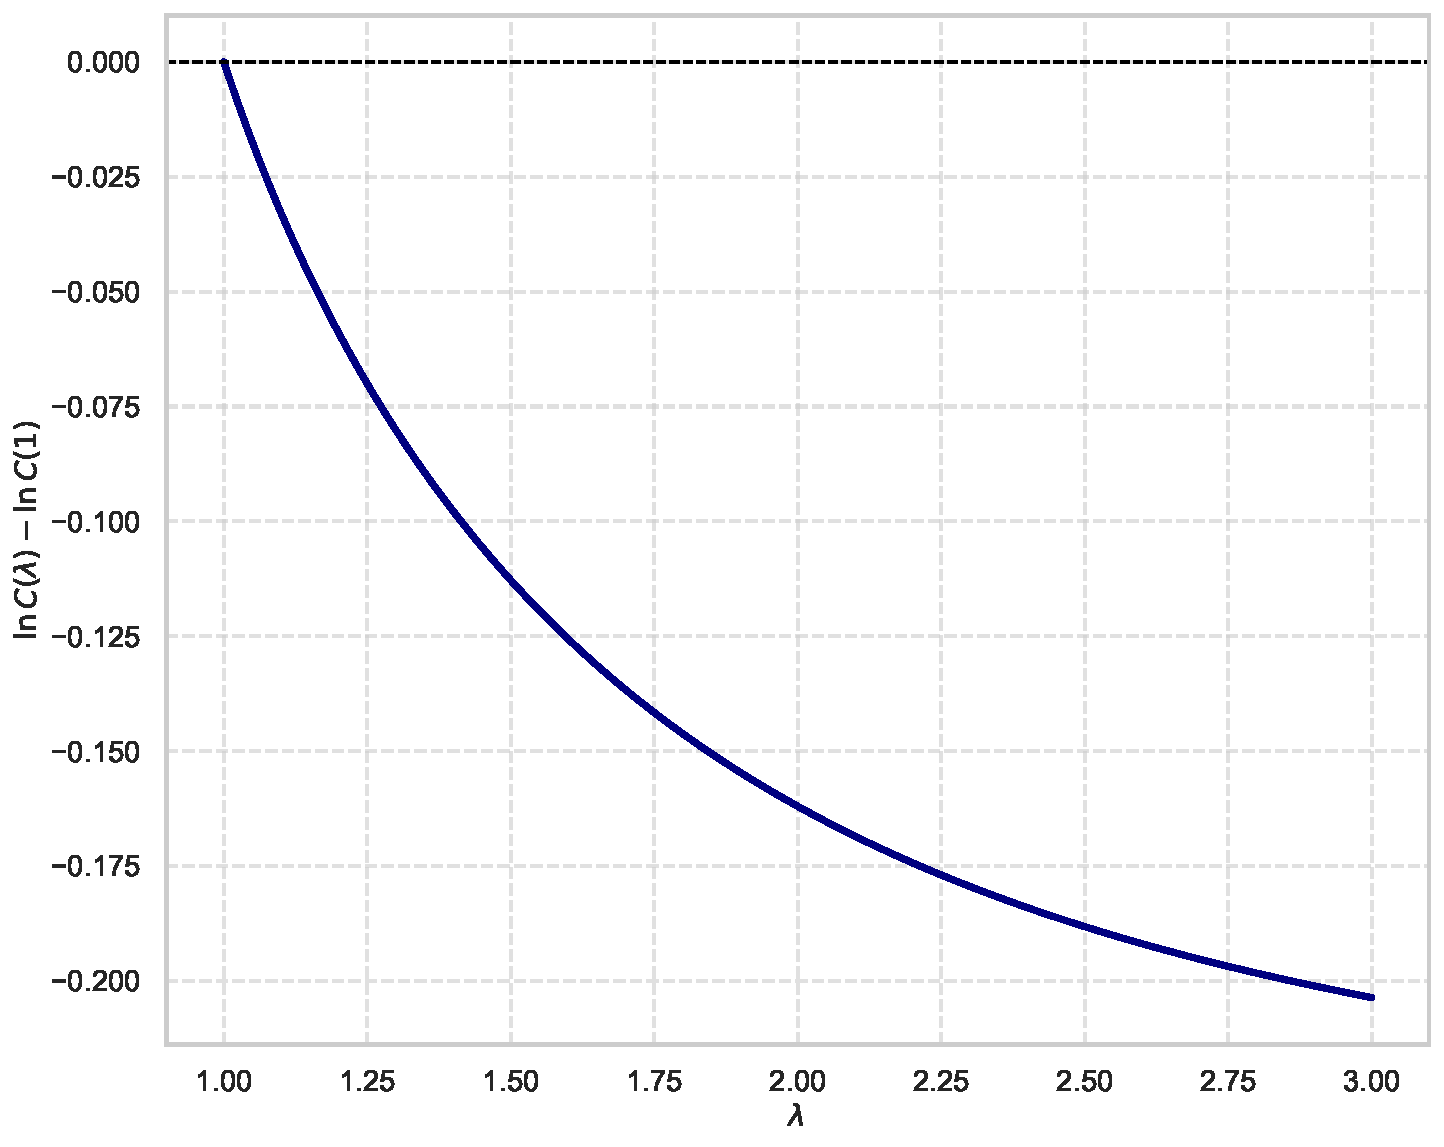
\includegraphics[width=0.5\linewidth]{figs/welfare_change_lambda.pdf}
    \caption{Caption}
    \label{fig:enter-label}
\end{figure}



\bibliography{bib/references}

\appendix

\section{Mathematical derivations}\label{sec:math}

\subsection{Proof of proposition 1}\label{sec:proof-1}

\paragraph{Part (a)}

\begin{proof}

First, recall that $\ln C = \ln (A_H L) - \ln P$, with $P = [\alpha + (1-\alpha) P_F^{-(\rho-1)}]^{-\frac{1}{\rho-1}}$. Therefore,  $\ln dC/d \ln \lambda = - \ln dP/d \ln \lambda$. We can write:

\begin{equation*}
    \frac{d \ln P}{d \ln \lambda} = \frac{(1-\alpha) P_F^{-(\rho-1)}}{P^{-(\rho-1)}} \times \frac{d P_F / P_F}{d \ln \lambda} = S_F \times \frac{d \ln P_F}{d \ln \lambda} 
\end{equation*}

\noindent where $S_F$ is the expenditure sure of consumers in foreign goods. Write the price of the foreign good and the cutoff point $\omega^*$ as a function of $\lambda$:

\begin{eqnarray*}
    P_F(\lambda) &=&  \left[\int_0^1 p_{h}(\omega)^{-(\sigma-1)}d\omega \right]^{-\frac{1}{\sigma-1}} \\
    &=& \left[\int_0^{\omega^*(\lambda)} p_{fh}(\omega)^{-(\sigma-1)}d\omega + \int_{\omega^*(\lambda)}^1 p_{rh}(\omega)^{-(\sigma-1)}d\omega \right]^{-\frac{1}{\sigma-1}} \\
    &=& \left[ (\lambda \mu c_f)^{-(\sigma-1)} \int_0^{\omega^*(\lambda)} \tau_{fh}(\omega)^{-(\sigma-1)}d\omega + (\mu^2 c_f)^{-(\sigma-1)}\int_{\omega^*(\lambda)}^1 \tau_{fh}^R(\omega)^{-(\sigma-1)}d\omega \right]^{-\frac{1}{\sigma-1}} \\    
    &=& \left[ (\lambda \mu c_f)^{-(\sigma-1)} \int_0^{\omega^*(\lambda)} \tau_{fh}(\omega)^{-(\sigma-1)}d\omega + (\mu^2 c_f)^{-(\sigma-1)}\int_{\omega^*(\lambda)}^1 \tau_{fh}^R(\omega)^{-(\sigma-1)}d\omega \right]^{-\frac{1}{\sigma-1}} \\    
    &=& \left[ P_{fh}(\lambda)^{-(\sigma-1)} + P_{rh}(\lambda)^{-(\sigma-1)} \right]^{-\frac{1}{\sigma-1}} 
\end{eqnarray*}

\noindent where $P_{ih}(\lambda)$ for $i \in \{f,r\}$ denote the average prices of varieties sourced directly from $f$ or through resourcing. Let $A(\lambda)=P_{fh}(\lambda)^{-(\sigma-1)}$. Then, the marginal impact of $\lambda$ on $P_F$ is:

\begin{eqnarray*}
    \frac{d \ln P_F(\lambda)}{d \ln\lambda} &=& \frac{\lambda}{P_F(\lambda)} P_F(\lambda)^{\sigma} \left[ \frac{\mathcal{A(\lambda)}}{\lambda} + [\lambda \mu c_f \tau_{fh}(\omega^*)]^{-(\sigma-1)}  \frac{d\omega^*(\lambda)}{d \lambda} - [\mu^2 c_f \tau^R_{fh}(\omega^*)]^{-(\sigma-1)}  \frac{d\omega^*(\lambda)}{d \lambda} \right] = s_{fh}(\lambda)
\end{eqnarray*}

\noindent where the last equally follows from the fact that, at the cut-off point, $\mu \tau^R_{fh}(\omega^*) = \lambda \tau_{fh}(\omega^*)$ and $s_{fh}(\lambda) = \left( \frac{P_{hf}(\lambda)}{P_F(\lambda)} \right)^{-(\sigma-1)}$ is the share of total expenditure on foreign goods spent on goods shipped directly from $f$ to $h$. Therefore, the elasticity of welfare with respect to the scaling factor $\lambda$ is:

\begin{equation}
    \frac{d \ln C(\lambda)}{d\ln \lambda} = - S_F(\lambda) \times s_{fh}(\lambda)
\end{equation}

\noindent which results in the first part of the proof.
\end{proof}

\paragraph{Part (b)} Since wages and population are constant,  $\ln C(\lambda') - \ln C(\lambda) =  -[\ln P(\lambda') - \ln P(\lambda)]$. By the fundamental theorem of calculus:

\begin{equation*}
    \ln C(\lambda') - \ln C(\lambda) =  -\int_\lambda^{\lambda'} \frac{d \ln P(\tilde{\lambda})}{d \ln \tilde{\lambda}} d \ln \tilde{\lambda} = - \int_\lambda^{\lambda'} S_F(\tilde{\lambda}) \times s_{fh}(\tilde{\lambda})   d \ln \tilde{\lambda} = - \int_\lambda^{\lambda'} \frac{S_F(\tilde{\lambda}) \times s_{fh}(\tilde{\lambda})}{\tilde{\lambda}}   d \tilde{\lambda}   
\end{equation*}



\end{document}
